\documentclass{article}

\usepackage[preprint]{corl_2026}

\usepackage[utf8]{inputenc}
\usepackage[T1]{fontenc}
\usepackage{amsmath,amssymb,bm}
\usepackage{booktabs}
\usepackage{graphicx}
\usepackage{tikz}
\usetikzlibrary{arrows.meta,positioning,calc,fit,backgrounds,decorations.markings}
\usepackage{pgfplots}
\pgfplotsset{compat=1.18}
\usepackage{listings}
\usepackage{xcolor}
\usepackage{microtype}

% ---------- notation ----------
\newcommand{\R}{\mathbb{R}}
\newcommand{\T}{\mathsf{T}}
\newcommand{\des}{\mathrm{des}}
\newcommand{\Kp}{K_p}
\newcommand{\Kd}{K_d}
\newcommand{\vq}{q}
\newcommand{\code}[1]{\texttt{#1}}
\newcommand{\subl}[1]{{\scriptsize\color{black!60}#1}}

% ---------- colours used in figures ----------
\definecolor{osctrain}{HTML}{1F6F8B}
\definecolor{osceval}{HTML}{B8571C}
\definecolor{band}{HTML}{E7EEF1}
\definecolor{bandlow}{HTML}{F1F1EE}
\definecolor{codebg}{HTML}{F4F5F4}

\lstset{
  language=Python,
  basicstyle=\ttfamily\scriptsize,
  commentstyle=\color{black!55}\itshape,
  keywordstyle=\bfseries,
  backgroundcolor=\color{codebg},
  frame=single, framerule=0pt, framesep=4pt,
  columns=fullflexible, keepspaces=true,
  breaklines=true, showstringspaces=false,
  xleftmargin=4pt, xrightmargin=4pt,
}

\tikzset{
  blk/.style={draw, rounded corners=2pt, minimum height=8mm, minimum width=18mm, align=center, font=\small, inner sep=3pt},
  sub/.style={font=\scriptsize\color{black!60}},
  arr/.style={-{Latex[length=2mm]}, thick},
  darr/.style={-{Latex[length=2mm]}, thick, dashed},
}

\title{From a Desired End-Effector Pose to Joint Torques:\\ The Relative Cartesian Operational-Space Controller in OmniReset}

\author{
  Tri Wahyu Guntara\\
  Tutorial notes on the UWLab OmniReset code base\\
}

\begin{document}
\maketitle

\begin{abstract}
The reinforcement-learning policies in the OmniReset peg-insertion task do not command joint angles or joint torques. They command a small displacement of the end effector, and a controller converts that displacement into the torques applied at the six joints of a UR5e arm. This tutorial derives that controller from first principles. We construct the desired pose from the policy action, define the position and orientation errors, introduce the geometric Jacobian, write the task-space proportional--derivative law, and show by the principle of virtual work why the transposed Jacobian maps a task-space force to joint torques. We then discuss the gains, the two control rates, the actuator layer, and what the controller deliberately omits relative to the full operational-space formulation. Each equation is mapped to the corresponding lines of the implementation.
\end{abstract}

\keywords{Operational-space control, Jacobian transpose, Sim-to-real, Reinforcement learning}

%==============================================================================
\section{The Pipeline at a Glance}
\label{sec:overview}

The policy in the OmniReset peg-insertion task~\cite{omnireset2026} outputs a small displacement of the end effector, and a controller is responsible for producing the joint torques that realise that displacement. The controller is a \emph{relative Cartesian operational-space controller}: relative, because the policy specifies a change of pose rather than an absolute pose; Cartesian, because the specification lives in the three-dimensional workspace rather than in joint space; and operational-space, because the control law is written in terms of a force on the end effector that is then mapped to the joints~\cite{khatib1987unified}.

Figure~\ref{fig:pipeline} shows the whole chain. Two rates are involved. The policy runs once every $0.1$\,s and produces a new desired pose. Within that interval the physics engine advances twelve times, and at every one of those steps the controller recomputes the torques from the current state and the held desired pose.

\begin{figure}[b]
\centering
\resizebox{\linewidth}{!}{%
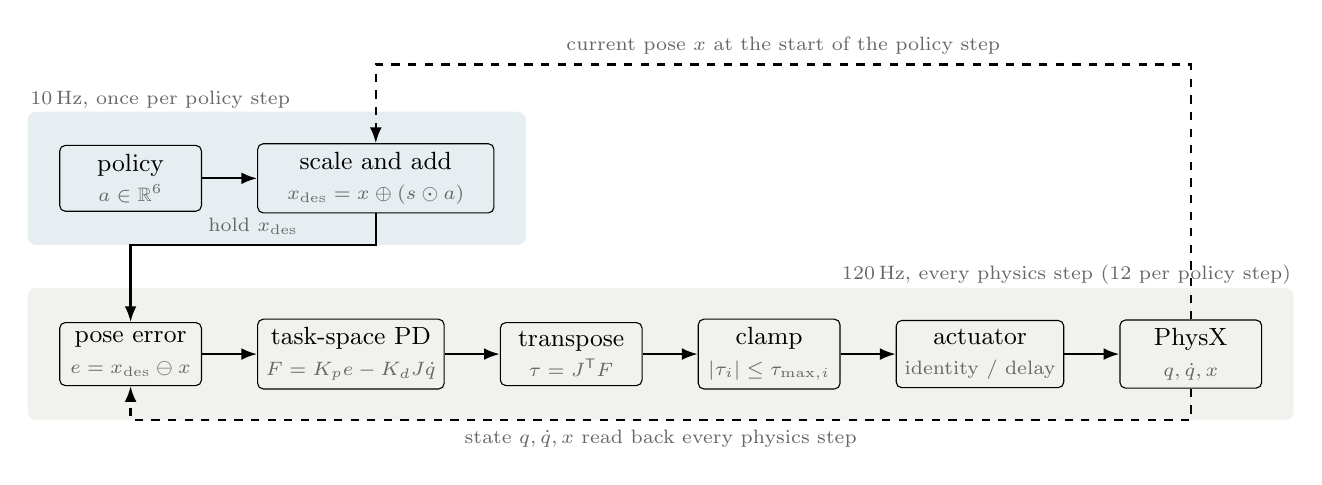
\begin{tikzpicture}[node distance=6mm and 7mm]
  % 10 Hz band
  \node[blk] (pol) {policy\\ \subl{$a\in\R^6$}};
  \node[blk, right=of pol, minimum width=30mm] (add) {scale and add\\ \subl{$x_\des = x \oplus (s\odot a)$}};
  % 120 Hz band
  \node[blk, below=14mm of pol] (err) {pose error\\ \subl{$e = x_\des \ominus x$}};
  \node[blk, right=of err] (pd) {task-space PD\\ \subl{$F=\Kp e-\Kd J\dot q$}};
  \node[blk, right=of pd] (jt) {transpose\\ \subl{$\tau = J^\T F$}};
  \node[blk, right=of jt] (cl) {clamp\\ \subl{$|\tau_i|\le\tau_{\max,i}$}};
  \node[blk, right=of cl] (act) {actuator\\ \subl{identity / delay}};
  \node[blk, right=of act] (phx) {PhysX\\ \subl{$q,\dot q,x$}};
  % arrows
  \draw[arr] (pol) -- (add);
  \draw[arr] (add.south) -- ++(0,-4mm) -| node[sub, pos=0.25, above] {hold $x_\des$} (err.north);
  \draw[arr] (err) -- (pd);
  \draw[arr] (pd) -- (jt);
  \draw[arr] (jt) -- (cl);
  \draw[arr] (cl) -- (act);
  \draw[arr] (act) -- (phx);
  \draw[darr] (phx.south) -- ++(0,-4mm) -| node[sub, pos=0.25, below] {state $q,\dot q,x$ read back every physics step} (err.south);
  \draw[darr] (phx.north) |- ($(add.north)+(0,10mm)$) node[sub, pos=0.75, above] {current pose $x$ at the start of the policy step} -- (add.north);
  % bands
  \begin{scope}[on background layer]
    \node[fill=band, rounded corners=3pt, fit=(pol)(add), inner sep=4mm, label={[sub, anchor=south west, inner sep=1pt]north west:10\,Hz, once per policy step}] {};
    \node[fill=bandlow, rounded corners=3pt, fit=(err)(phx), inner sep=4mm, label={[sub, anchor=south east, inner sep=1pt]north east:120\,Hz, every physics step (12 per policy step)}] {};
  \end{scope}
\end{tikzpicture}}
\caption{The control chain. The upper band runs once per policy step and only decides \emph{where} the end effector should be. The lower band runs at the physics rate and decides \emph{how hard to push} toward that place. Dashed arrows carry state read from the simulator.}
\label{fig:pipeline}
\end{figure}

%==============================================================================
\section{Frames and Notation}
\label{sec:notation}

Throughout, all poses, velocities, forces, and Jacobians are expressed in the robot's \emph{base frame}, the frame of the UR5e's \code{base\_link}. The end effector is the \code{wrist\_3\_link}, the flange to which the gripper is bolted; the gripper itself is not part of the controlled chain. The six arm joints are, in order, the shoulder pan, shoulder lift, elbow, and three wrist joints.

Let $q\in\R^6$ be the vector of arm joint angles and $\dot q$ its time derivative. The end-effector pose is the pair $x=(p,Q)$, where $p\in\R^3$ is the position and $Q$ is a unit quaternion, stored in $(x,y,z,w)$ order as elsewhere in the code base. A rotation can equally be written as a rotation vector $\theta\hat n\in\R^3$, the product of an angle and a unit axis; the controller moves between the two representations freely. $\Delta x\in\R^6$ denotes a small pose change, with its first three entries a translation and its last three a rotation vector. The subscript $\des$ marks a desired quantity, $\Kp,\Kd\in\R^{6\times6}$ are diagonal gain matrices, and $J(q)\in\R^{6\times6}$ is the geometric Jacobian.

Because the position and orientation both have three degrees of freedom, every task-space quantity in this controller is six-dimensional, and the arm has exactly six joints. The Jacobian is therefore square. This coincidence simplifies the exposition but is not essential: the control law below is valid for any number of joints.

%==============================================================================
\section{From Action to Desired Pose}
\label{sec:target}

The policy emits an action $a\in\R^6$ whose entries are nominally of unit scale. The first operation multiplies it elementwise by a fixed scale vector $s$, which converts a dimensionless network output into metres and radians:
\begin{equation}
  \Delta x = s\odot a, \qquad s_{\text{train}} = (0.02,\,0.02,\,0.02,\;0.02,\,0.02,\,0.2).
\end{equation}
During the first training stage a unit action therefore requests a $2$\,cm translation along any axis, a rotation of $0.02$\,rad (about $1.1^\circ$) about the base $x$ or $y$ axes, and a rotation of $0.2$\,rad (about $11.5^\circ$) about the base $z$ axis. The larger allowance about $z$ reflects the task: aligning a peg with a hole mostly requires turning the tool about its own axis.

The translational part of the desired pose is simply the current position plus the commanded displacement,
\begin{equation}
  p_\des = p + \Delta x_{1:3}.
\end{equation}
The rotational part requires more care, because rotations do not add. The last three entries of $\Delta x$ form a rotation vector $\mathbf r=\Delta x_{4:6}$. Its magnitude is the rotation angle and its direction is the rotation axis,
\begin{equation}
  \theta = \lVert\mathbf r\rVert, \qquad \hat n = \mathbf r/\theta \quad (\theta>10^{-6}),
\end{equation}
and the corresponding unit quaternion is obtained from the exponential map,
\begin{equation}
  \Delta Q = \big(\hat n\sin\tfrac{\theta}{2},\;\cos\tfrac{\theta}{2}\big).
\end{equation}
When $\theta$ is below the threshold, the axis is undefined and the code substitutes the identity rotation $\Delta Q=(0,0,0,1)$. The desired orientation is then the composition
\begin{equation}
  Q_\des = \Delta Q\otimes Q,
  \label{eq:qdes}
\end{equation}
where $\otimes$ is the quaternion (Hamilton) product. The order matters. Multiplying on the left applies $\Delta Q$ \emph{after} $Q$ and therefore expresses the rotation in the base frame: a positive $\mathbf r$ about the base $z$ axis always turns the tool about the vertical, regardless of how the tool is currently oriented. Had the delta been multiplied on the right, it would have been interpreted in the tool's own frame.

\paragraph{Why ``relative'' is a design decision.}
Because $x_\des$ is rebuilt from the \emph{measured} pose at every policy step, the target can never run away from the robot. If contact with the hole stops the peg, the next policy step starts again from where the peg actually is, and the accumulated error is wiped out. This is what makes the scheme safe for contact-rich insertion: a stuck end effector never results in an ever-growing restoring force.

%==============================================================================
\section{The Pose Error}
\label{sec:error}

At every physics step the controller reads the current pose $x=(p,Q)$ and compares it with the held target. The position error is the plain difference
\begin{equation}
  e_p = p_\des - p \in\R^3.
\end{equation}
The orientation error is the rotation that takes the current orientation to the desired one. In quaternion form it is
\begin{equation}
  Q_e = Q_\des\otimes Q^{-1},
\end{equation}
which satisfies $Q_e\otimes Q = Q_\des$, as required. This quaternion is converted back to a rotation vector by the logarithmic map, the inverse of the construction in Section~\ref{sec:target}:
\begin{equation}
  e_o = \log(Q_e) = 2\,\operatorname{atan2}\!\big(\lVert\mathbf v\rVert, w\big)\,\frac{\mathbf v}{\lVert\mathbf v\rVert}, \qquad Q_e=(\mathbf v,w).
\end{equation}
For small misalignments, $e_o$ is approximately twice the vector part of $Q_e$, and it behaves like an ordinary three-dimensional error signal: its direction is the axis about which the tool must turn and its magnitude is the remaining angle. The full six-dimensional error is the concatenation
\begin{equation}
  e = \begin{bmatrix} e_p\\ e_o\end{bmatrix}\in\R^6.
\end{equation}
Immediately after a policy step, before the arm has moved, the error equals the commanded delta, $e=\Delta x$. As the arm moves, the error shrinks toward zero.

%==============================================================================
\section{The Jacobian}
\label{sec:jacobian}

The geometric Jacobian links joint velocities to the linear and angular velocity of the end effector~\cite{siciliano2009robotics,lynch2017modern},
\begin{equation}
  \begin{bmatrix} v\\ \omega\end{bmatrix} = J(q)\,\dot q, \qquad J(q)\in\R^{6\times6}.
\end{equation}
Each column of $J$ is the end-effector twist produced by unit velocity at one joint while the others are held still. For a revolute joint $i$ with axis $\hat z_i$ through the point $o_i$, that column is
\begin{equation}
  J_{:,i} = \begin{bmatrix} \hat z_i\times(p-o_i)\\ \hat z_i\end{bmatrix},
\end{equation}
where $p$ is the end-effector position. The cross product expresses the familiar fact that rotating about a distant axis sweeps the tool through a large arc, whereas rotating about a nearby axis barely moves it.

The controller does not query the physics engine for this matrix. It evaluates a closed-form expression derived from the UR5e's kinematic parameters, with the parameters replaced by values measured on the physical robot during calibration. This choice is deliberate. The real robot's controller uses exactly the same analytical Jacobian, so using it in simulation removes one source of discrepancy between the two. For the same reason the end-effector velocity entering the damping term is not read from the simulator but computed as $J\dot q$ from the measured joint velocities, which keeps the velocity and the Jacobian mutually consistent.

%==============================================================================
\section{The Task-Space PD Law}
\label{sec:pd}

With an error and a velocity in hand, the controller computes a \emph{virtual wrench}, a force and a moment that one would like to apply to the end effector:
\begin{equation}
  F = \Kp\,e + \Kd\big(\dot x_\des - J\dot q\big), \qquad \dot x_\des = 0.
  \label{eq:pd}
\end{equation}
The proportional term pulls the end effector toward the target in proportion to the remaining error, exactly as a spring would. The derivative term opposes the end-effector velocity, as a damper would. Because the target is held constant between policy steps, the desired velocity is zero and the damping term reduces to $-\Kd J\dot q$. The analogy is therefore literal: the controller behaves as if six springs and six dampers, one per Cartesian direction, connected the tool to an invisible anchor at $x_\des$.

Both gain matrices are diagonal, so each direction is tuned independently. The stiffness matrix is specified directly; the damping is derived from it through a \emph{damping ratio} $\zeta$,
\begin{equation}
  \Kd = 2\zeta\sqrt{\Kp}\quad\text{elementwise}.
  \label{eq:kd}
\end{equation}
To see where this comes from, consider a single direction and suppose, for the moment, that the end effector behaved as a point of unit mass. Its motion would obey
\begin{equation}
  \ddot e + \Kd\dot e + \Kp e = 0,
\end{equation}
the equation of a damped harmonic oscillator with natural frequency $\omega_n=\sqrt{\Kp}$. Writing $\Kd=2\zeta\omega_n$ gives the standard form $\ddot e+2\zeta\omega_n\dot e+\omega_n^2 e=0$, in which $\zeta$ alone decides the shape of the response: $\zeta<1$ oscillates, $\zeta=1$ returns to zero as fast as possible without overshooting, and $\zeta>1$ returns more slowly and without overshoot. Section~\ref{sec:gains} shows what the two gain sets used in OmniReset look like under this model.

%==============================================================================
\section{From Task-Space Force to Joint Torque}
\label{sec:transpose}

The wrench $F$ is a fiction: no actuator pushes on the wrist. What the robot can do is apply a torque $\tau_i$ at each joint. The question is which joint torques are equivalent to the desired wrench, and the answer is given by the principle of virtual work.

Suppose the joints move by an infinitesimal displacement $\delta q$. The end effector then moves by $\delta x=J\delta q$. The work done by the joint torques is $\tau^\T\delta q$; the work that the wrench would do through the same motion is $F^\T\delta x$. For the two to be equivalent, the work must agree for \emph{every} possible $\delta q$:
\begin{equation}
  \tau^\T\delta q = F^\T J\,\delta q\quad\forall\,\delta q
  \quad\Longrightarrow\quad
  \tau = J^\T F.
  \label{eq:transpose}
\end{equation}
This is the central identity of operational-space control. The transpose of the matrix that maps joint velocities to end-effector velocities is the matrix that maps end-effector forces back to joint torques. No matrix inversion is required, and the formula remains valid even when $J$ is singular, which is one reason the transpose law is preferred over inverse-kinematics schemes for contact tasks.

The final operation is a safety clamp. Each component of $\tau$ is limited to the torque the corresponding joint can deliver,
\begin{equation}
  \tau_i \leftarrow \operatorname{clip}\big(\tau_i,-\tau_{\max,i},\tau_{\max,i}\big), \qquad
  \tau_{\max} = (150,150,150,28,28,28)\ \mathrm{N\cdot m}.
\end{equation}
The three large joints of the UR5e are rated for $150$\,N$\cdot$m and the three wrist joints for $28$\,N$\cdot$m. Clamping after the transpose, rather than clamping $F$, means that the limit is applied where it physically exists, at the joint, although it also means that a saturated joint changes the direction of the realised wrench.

%==============================================================================
\section{A Planar Example}
\label{sec:planar}

The six-dimensional case is hard to picture, but a two-link planar arm shows everything that matters. Let the links have lengths $\ell_1,\ell_2$ and joint angles $\theta_1,\theta_2$, with $\theta_2$ measured relative to the first link. The tip position is
\begin{equation}
  p = \begin{bmatrix} \ell_1\cos\theta_1+\ell_2\cos(\theta_1+\theta_2)\\ \ell_1\sin\theta_1+\ell_2\sin(\theta_1+\theta_2)\end{bmatrix},
\end{equation}
and differentiating with respect to the joint angles gives the Jacobian
\begin{equation}
  J = \begin{bmatrix}
    -\ell_1\sin\theta_1-\ell_2\sin(\theta_1+\theta_2) & -\ell_2\sin(\theta_1+\theta_2)\\
    \phantom{-}\ell_1\cos\theta_1+\ell_2\cos(\theta_1+\theta_2) & \phantom{-}\ell_2\cos(\theta_1+\theta_2)
  \end{bmatrix}.
\end{equation}
Now take the configuration in Figure~\ref{fig:planar}, with the arm stretched horizontally, $\theta_1=\theta_2=0$. The Jacobian collapses to
\begin{equation}
  J = \begin{bmatrix} 0 & 0\\ \ell_1+\ell_2 & \ell_2\end{bmatrix}, \qquad
  J^\T = \begin{bmatrix} 0 & \ell_1+\ell_2\\ 0 & \ell_2\end{bmatrix}.
\end{equation}
Suppose the controller wants to push the tip upward with force $F=(0,F_y)$. Then
\begin{equation}
  \tau = J^\T F = \begin{bmatrix} (\ell_1+\ell_2)F_y\\ \ell_2 F_y\end{bmatrix}.
\end{equation}
Each joint receives the force times its lever arm to the tip, which is exactly the torque a static force at the tip would exert on that joint. The shoulder, being farther away, must work harder than the elbow. If instead the controller wants to push along the arm, $F=(F_x,0)$, the result is $\tau=0$: the stretched arm cannot move in that direction, so no torque can help, and the transpose law quietly produces none. An inverse-Jacobian controller would have divided by zero at the same configuration.

\begin{figure}[t]
\centering
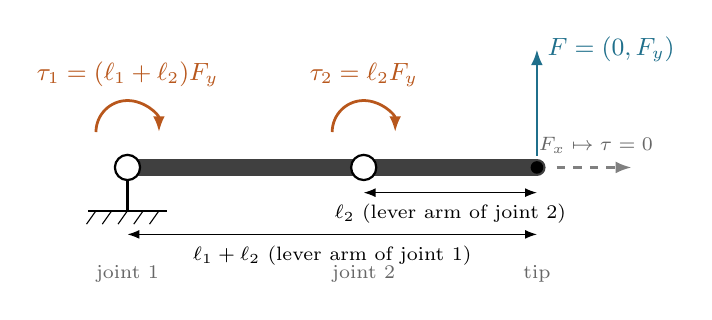
\begin{tikzpicture}[scale=1.0]
  % ground
  \draw[thick] (-0.5,-0.55) -- (0.5,-0.55);
  \foreach \x in {-0.4,-0.2,0,0.2,0.4} \draw (\x,-0.55) -- (\x-0.12,-0.72);
  \draw[thick] (0,-0.55) -- (0,0);
  % links
  \draw[line width=2.2mm, line cap=round, black!75] (0,0) -- (3,0);
  \draw[line width=2.2mm, line cap=round, black!75] (3,0) -- (5.2,0);
  % joints
  \fill[white] (0,0) circle (0.16); \draw[thick] (0,0) circle (0.16);
  \fill[white] (3,0) circle (0.16); \draw[thick] (3,0) circle (0.16);
  \fill (5.2,0) circle (0.08);
  % force
  \draw[arr, osctrain, line width=1pt] (5.2,0.15) -- (5.2,1.5) node[right, font=\small] {$F=(0,F_y)$};
  % torque arcs
  \draw[arr, osceval, line width=1pt] (-0.4,0.45) arc[start angle=180, end angle=0, radius=0.4];
  \node[osceval, font=\small, above] at (0,0.9) {$\tau_1=(\ell_1+\ell_2)F_y$};
  \draw[arr, osceval, line width=1pt] (2.6,0.45) arc[start angle=180, end angle=0, radius=0.4];
  \node[osceval, font=\small, above] at (3,0.9) {$\tau_2=\ell_2 F_y$};
  % dimensions
  \draw[{Latex[length=1.5mm]}-{Latex[length=1.5mm]}] (3,-0.32) -- (5.2,-0.32);
  \node[font=\scriptsize, below] at (4.1,-0.34) {$\ell_2$ (lever arm of joint 2)};
  \draw[{Latex[length=1.5mm]}-{Latex[length=1.5mm]}] (0,-0.85) -- (5.2,-0.85);
  \node[font=\scriptsize, below] at (2.6,-0.87) {$\ell_1+\ell_2$ (lever arm of joint 1)};
  % along-arm note
  \draw[arr, black!50, dashed] (5.45,0) -- (6.4,0);
  \node[font=\scriptsize, black!60, above] at (5.95,0.05) {$F_x\mapsto\tau=0$};
  % labels
  \node[font=\scriptsize, black!60] at (0,-1.35) {joint 1};
  \node[font=\scriptsize, black!60] at (3,-1.35) {joint 2};
  \node[font=\scriptsize, black!60] at (5.2,-1.35) {tip};
\end{tikzpicture}
\caption{The transpose law on a two-link arm. The upward force at the tip is converted into joint torques equal to the force times each joint's lever arm. A force along the stretched arm maps to zero torque, because the arm cannot move that way.}
\label{fig:planar}
\end{figure}

%==============================================================================
\section{Gains, Damping Ratios, and the Step Response}
\label{sec:gains}

OmniReset uses two gain sets, listed in Table~\ref{tab:gains}. The first, used throughout the initial training stage, is deliberately soft and heavily overdamped. The second, used for evaluation and for the real robot, is five times stiffer in translation and critically damped. During fine-tuning a curriculum interpolates from the first to the second.

\begin{table}[t]
\centering
\caption{The two gain sets. The damping follows from the stiffness and the damping ratio by Eq.~\eqref{eq:kd}. Torque limits are $150$\,N$\cdot$m on joints 1--3 and $28$\,N$\cdot$m on joints 4--6 in both settings.}
\label{tab:gains}
\small
\begin{tabular}{@{}lrrrr@{}}
\toprule
 & \multicolumn{2}{c}{Training (stage 1)} & \multicolumn{2}{c}{Evaluation / real robot}\\
\cmidrule(lr){2-3}\cmidrule(lr){4-5}
Quantity & $x,y,z$ & $r_x,r_y,r_z$ & $x,y,z$ & $r_x,r_y,r_z$\\
\midrule
Stiffness $\Kp$            & 200   & 3     & 1000  & 50\\
Damping ratio $\zeta$      & 3.0   & 1.0   & 1.0   & 1.0\\
Damping $\Kd=2\zeta\sqrt{\Kp}$ & 84.9 & 3.46 & 63.2 & 14.1\\
Action scale $s$           & 0.02\,m & 0.02, 0.02, 0.2\,rad & 0.01, 0.01, 0.002\,m & 0.02, 0.02, 0.2\,rad\\
\bottomrule
\end{tabular}
\end{table}

The unit-mass model of Section~\ref{sec:pd} lets us compare the two settings. For the training gains in translation, the characteristic equation $s^2+84.9\,s+200=0$ has roots near $-2.4$ and $-82$. The fast root dies out almost immediately; the slow root gives a time constant of about $0.4$\,s. For the evaluation gains, $s^2+63.2\,s+1000=0$ has a double root at $-31.6$, a time constant of about $0.03$\,s.

Figure~\ref{fig:step} integrates the model numerically for a step of one action unit. The vertical rules mark the $0.1$\,s policy period. With the training gains, the end effector has covered only about $19\%$ of the commanded $2$\,cm by the time the next action arrives; the commanded delta functions less as a position target than as a velocity command, which is a sensible thing for an exploring policy to control. With the evaluation gains, the arm completes about $82\%$ of the (smaller) step within one policy period, so the policy commands positions in a more literal sense. Under a heavier effective mass both curves slow down; the real arm's apparent mass varies with its configuration, which is the price of omitting the inertia matrix discussed in Section~\ref{sec:osc}.

\begin{figure}[t]
\centering
\begin{tikzpicture}
\begin{axis}[
  width=0.9\linewidth, height=0.45\linewidth,
  xlabel={time since the policy step [s]}, ylabel={fraction of step completed},
  xmin=0, xmax=1, ymin=0, ymax=1.08,
  ytick={0,0.25,0.5,0.75,1}, yticklabels={0\%,25\%,50\%,75\%,100\%},
  xtick={0,0.1,...,1.0}, xticklabel style={/pgf/number format/fixed, /pgf/number format/precision=1},
  grid=both, grid style={black!12},
  minor x tick num=0,
  legend style={font=\footnotesize, draw=none, fill=none, at={(0.5,-0.22)}, anchor=north, legend columns=2, /tikz/every even column/.append style={column sep=6pt}},
  tick label style={font=\footnotesize}, label style={font=\footnotesize},
]
  \addplot[osctrain, thick] table[x=t, y=train] {step_response.dat};
  \addlegendentry{Training, $\Kp=200$, $\zeta=3$, $m=1$}
  \addplot[osceval, thick, dashed] table[x=t, y=eval] {step_response.dat};
  \addlegendentry{Evaluation, $\Kp=1000$, $\zeta=1$, $m=1$}
  \addplot[osctrain, thin, dotted] table[x=t, y=train4] {step_response.dat};
  \addlegendentry{Training, $m=4$}
  \addplot[osceval, thin, dotted] table[x=t, y=eval4] {step_response.dat};
  \addlegendentry{Evaluation, $m=4$}
  \addplot[black!50, dashed, thin, forget plot] coordinates {(0,1) (1,1)};
  \addplot[osctrain, only marks, mark=*, mark size=1.6pt, forget plot] coordinates {(0.1,0.1924)};
  \addplot[osceval, only marks, mark=*, mark size=1.6pt, forget plot] coordinates {(0.1,0.8245)};
  \draw[osctrain, thin] (axis cs:0.1,0.1924) -- (axis cs:0.22,0.10);
  \node[font=\scriptsize, anchor=west, osctrain] at (axis cs:0.22,0.10) {19\% at 0.1\,s};
  \draw[osceval, thin] (axis cs:0.1,0.8245) -- (axis cs:0.22,0.62);
  \node[font=\scriptsize, anchor=west, osceval] at (axis cs:0.22,0.62) {82\% at 0.1\,s};
\end{axis}
\end{tikzpicture}
\caption{Fraction of a commanded translation step completed as a function of time, for the two gain sets, under an effective end-effector mass $m$ of $1$\,kg (solid, dashed) and $4$\,kg (dotted). The grid lines at multiples of $0.1$\,s are policy steps.}
\label{fig:step}
\end{figure}

The rotational gains deserve a remark. A stiffness of $3$\,N$\cdot$m/rad with the training set is tiny: an orientation error of a full radian produces only $3$\,N$\cdot$m of moment at the wrist. This is intentional during exploration, since a compliant wrist survives collisions with the hole gracefully, and the fine-tuning curriculum raises the value to $50$\,N$\cdot$m/rad once the policy is competent.

%==============================================================================
\section{Timing: Two Control Rates}
\label{sec:timing}

The simulation runs at a time step of $1/120$\,s and the environment applies a \emph{decimation} of $12$, so the policy acts once every $12/120=0.1$\,s. Figure~\ref{fig:timing} lays the two clocks side by side. At each policy tick the desired pose is recomputed from the measured pose and then held constant, a zero-order hold. In between, the controller runs twelve times, each time with a fresh measurement of $q$, $\dot q$ and $x$ but the same $x_\des$.

\begin{figure}[t]
\centering
\resizebox{\linewidth}{!}{%
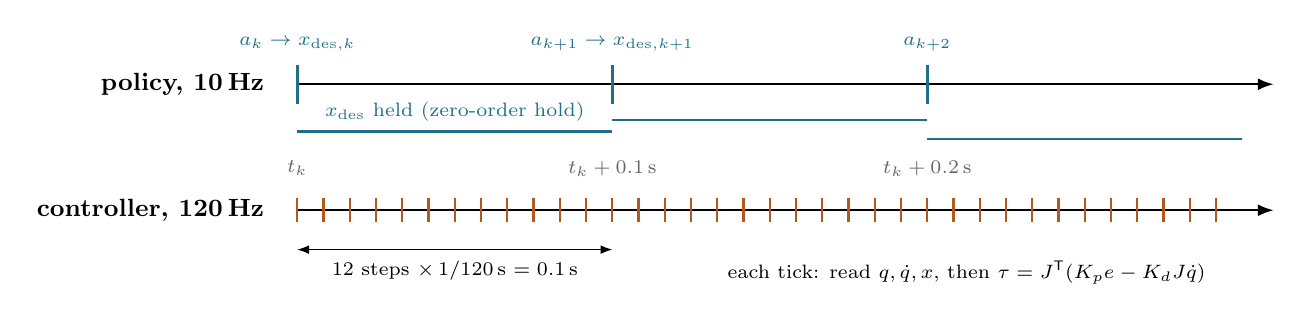
\begin{tikzpicture}[x=1cm]
  % policy axis
  \node[font=\small\bfseries, anchor=east] at (-0.3,1.6) {policy, 10\,Hz};
  \draw[arr] (0,1.6) -- (12.4,1.6);
  \foreach \x/\l in {0/{$a_k \to x_{\des,k}$}, 4/{$a_{k+1}\to x_{\des,k+1}$}, 8/{$a_{k+2}$}} {
    \draw[osctrain, line width=1.2pt] (\x,1.35) -- (\x,1.85);
    \node[osctrain, font=\scriptsize, above] at (\x,1.9) {\l};
  }
  % held target
  \draw[osctrain, thick] (0,1.0) -- (4,1.0);
  \draw[osctrain, thick] (4,1.15) -- (8,1.15);
  \draw[osctrain, thick] (8,0.9) -- (12,0.9);
  \node[osctrain, font=\scriptsize, above] at (2,1.0) {$x_\des$ held (zero-order hold)};
  % controller axis
  \node[font=\small\bfseries, anchor=east] at (-0.3,0) {controller, 120\,Hz};
  \draw[arr] (0,0) -- (12.4,0);
  \foreach \i in {0,...,35} { \draw[osceval, thick] ({\i/3},-0.15) -- ({\i/3},0.15); }
  \draw[{Latex[length=1.5mm]}-{Latex[length=1.5mm]}] (0,-0.5) -- (4,-0.5);
  \node[font=\scriptsize, below] at (2,-0.52) {12 steps $\times\, 1/120$\,s $= 0.1$\,s};
  \node[font=\scriptsize, below] at (8.5,-0.52) {each tick: read $q,\dot q,x$, then $\tau=J^\T(\Kp e-\Kd J\dot q)$};
  \foreach \x/\l in {0/{$t_k$}, 4/{$t_k+0.1$\,s}, 8/{$t_k+0.2$\,s}} \node[font=\scriptsize, black!60, below] at (\x,0.75) {\l};
\end{tikzpicture}}
\caption{The two clocks. A policy action fixes the target for the next twelve physics steps; the torque is recomputed at each of them from the latest measurement. The held target is drawn at a different height after each tick to emphasise that it is rebuilt from the measured pose, not accumulated.}
\label{fig:timing}
\end{figure}

Running the feedback loop at the physics rate rather than at the policy rate is what makes the soft gains workable. A spring-damper evaluated only ten times a second would be unstable for the damping values in Table~\ref{tab:gains}, because $\Kd\,\Delta t=84.9\times0.1\approx8.5$ far exceeds the stability margin of a discrete damper. At $\Delta t=1/120$\,s the same product is about $0.7$, which is comfortably stable.

%==============================================================================
\section{The Actuator Layer}
\label{sec:actuator}

In Isaac Lab~\cite{mittal2023orbit} the quantity produced by an action term is a \emph{target}, and an actuator model decides what the simulator finally receives. For a position-controlled robot the actuator would contain its own joint-level PD loop with its own stiffness and damping. The OmniReset arm sets both of those to zero. The effort target coming out of the operational-space controller is therefore passed to the physics engine unchanged, and the only PD loop in the system is the task-space one described above. Figure~\ref{fig:actuator} shows the layer in the two training stages.

\begin{figure}[t]
\centering
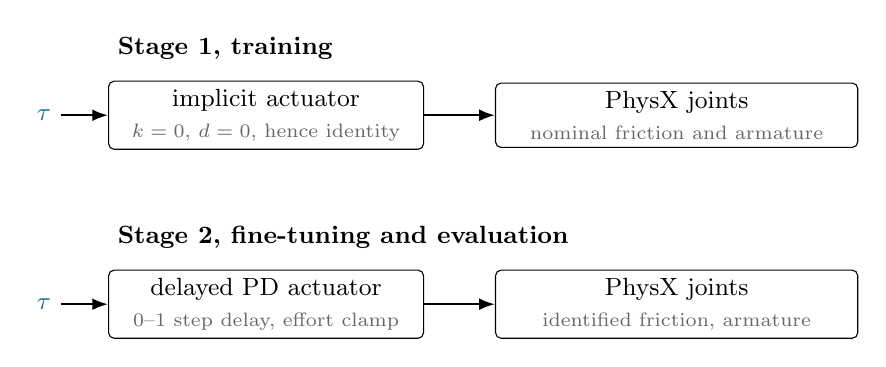
\begin{tikzpicture}[node distance=5mm and 9mm]
  \node[blk, minimum width=40mm] (a1) at (0,0) {implicit actuator\\ \subl{$k=0$, $d=0$, hence identity}};
  \node[blk, right=of a1, minimum width=46mm] (p1) {PhysX joints\\ \subl{nominal friction and armature}};
  \node[osctrain, font=\small, left=6mm of a1] (t1) {$\tau$};
  \draw[arr] (t1) -- (a1); \draw[arr] (a1) -- (p1);
  \node[font=\small\bfseries, anchor=south west] at ($(a1.north west)+(0,1.5mm)$) {Stage 1, training};
  \node[blk, minimum width=40mm] (a2) at (0,-2.4) {delayed PD actuator\\ \subl{0--1 step delay, effort clamp}};
  \node[blk, right=of a2, minimum width=46mm] (p2) {PhysX joints\\ \subl{identified friction, armature}};
  \node[osctrain, font=\small, left=6mm of a2] (t2) {$\tau$};
  \draw[arr] (t2) -- (a2); \draw[arr] (a2) -- (p2);
  \node[font=\small\bfseries, anchor=south west] at ($(a2.north west)+(0,1.5mm)$) {Stage 2, fine-tuning and evaluation};
\end{tikzpicture}
\caption{The actuator layer in the two training stages. In neither stage does the actuator add a joint-level PD term. The second stage inserts a one-step motor delay and loads the joint friction and rotor inertia identified on the physical arm, so that the same controller faces a more realistic plant.}
\label{fig:actuator}
\end{figure}

The second training stage replaces the implicit actuator by a \emph{delayed} one. Its joint-level gains are still zero, so it still does not add a PD term; what it adds is a delay of zero or one physics step between the torque being computed and its being applied, together with an explicit effort clamp. In the same stage a randomisation event writes the joint friction and armature values identified on the real UR5e~\cite{bjelonic2025pace} into the simulator, scaled by a factor drawn from a range that a curriculum widens as the policy's success rate permits. The controller itself does not know about any of this; it only notices that the plant has become harder to move.

%==============================================================================
\section{What the Controller Leaves Out}
\label{sec:osc}

Readers familiar with Khatib's operational-space formulation~\cite{khatib1987unified} will have noticed an omission. The complete law reads
\begin{equation}
  \tau = J^\T\Lambda(q)\big(\Kp e-\Kd J\dot q\big) + \mu(q,\dot q) + g(q),
\end{equation}
where $\Lambda(q)=\big(JM^{-1}J^\T\big)^{-1}$ is the task-space inertia matrix built from the joint-space mass matrix $M(q)$, and $\mu$ and $g$ compensate Coriolis, centrifugal, and gravitational effects. Pre-multiplying by $\Lambda$ makes the closed loop behave exactly like the unit-mass oscillator of Section~\ref{sec:pd} in every direction and every configuration. The OmniReset controller drops $\Lambda$, $\mu$, and $g$ entirely, so the law is
\begin{equation}
  \tau = J^\T\big(\Kp e-\Kd J\dot q\big)
\end{equation}
and nothing more. Three consequences follow.
\begin{enumerate}
  \item \textbf{The apparent stiffness depends on the configuration.} Without $\Lambda$, the same gain produces a fast response in directions where the arm is light and a slow one where it is heavy. This is why Figure~\ref{fig:step} shows two effective masses: no single curve describes the real arm.
  \item \textbf{Gravity must come from elsewhere.} In simulation the robot links are spawned with gravity disabled, so there is nothing to compensate. On the physical UR5e the manufacturer's firmware compensates gravity below the level at which torques are commanded, so again the controller need not.
  \item \textbf{Simulation and reality use the same equations.} This is the reason for the simplification. The controller running on the real robot is this same transpose PD law with the same analytical Jacobian and the same gains. A more sophisticated simulated controller would have trained the policy against a plant that behaves differently from the one it meets on deployment.
\end{enumerate}

%==============================================================================
\section{Mapping the Mathematics to the Code}
\label{sec:code}

The controller is implemented in the class \code{RelCartesianOSCAction} in the file \path{source/uwlab_tasks/uwlab_tasks/manager_based/manipulation/omnireset/mdp/actions/task_space_actions.py}. Its two methods correspond to the two bands of Figure~\ref{fig:pipeline}. The first runs once per policy step and implements Section~\ref{sec:target}:

\begin{lstlisting}
def process_actions(self, actions):
    scaled = actions * self._scale                          # dx = s * a
    ee_pos_b, ee_quat_b = self._get_ee_pose_root_frame()    # x = (p, Q) in the base frame
    self._ee_pos_des[:] = ee_pos_b + scaled[:, :3]          # p_des = p + dx[0:3]

    delta_rot = scaled[:, 3:6]                              # rotation vector r
    angle = torch.norm(delta_rot, dim=-1, keepdim=True)     # theta = |r|
    axis = delta_rot / angle      # guarded for theta ~ 0   # n = r / theta
    delta_quat = cat([axis * sin(angle / 2), cos(angle / 2)])   # dQ = (n sin, cos)
    self._ee_quat_des[:] = quat_mul(delta_quat, ee_quat_b)      # Q_des = dQ * Q
\end{lstlisting}

The second runs at every physics step and implements Sections~\ref{sec:error} through~\ref{sec:transpose} in order:

\begin{lstlisting}
def apply_actions(self):
    ee_pos_b, ee_quat_b = self._get_ee_pose_root_frame()
    joint_pos = self._asset.data.joint_pos[:, self._joint_ids]        # q
    joint_vel = self._asset.data.joint_vel[:, self._joint_ids]        # dq

    jacobian = compute_jacobian_analytical(joint_pos)                 # J(q), calibrated
    ee_vel = bmm(jacobian, joint_vel)                                 # xdot = J dq

    pos_error = self._ee_pos_des - ee_pos_b                           # e_p
    quat_error = quat_mul(self._ee_quat_des, quat_inv(ee_quat_b))     # Q_e = Q_des * Q^-1
    pose_error = cat([pos_error, axis_angle_from_quat(quat_error)])   # e = [e_p; log Q_e]

    task_force = self._kp * pose_error + self._kd * (-ee_vel)         # F = Kp e - Kd xdot
    joint_torques = bmm(jacobian.transpose(-1, -2), task_force)       # tau = J^T F
    joint_torques = clamp(joint_torques, -self._torque_max, self._torque_max)
    self._asset.set_joint_effort_target(joint_torques, joint_ids=self._joint_ids)
\end{lstlisting}

Two implementation details complete the picture. In the constructor the damping is derived from the stiffness exactly as in Eq.~\eqref{eq:kd}, and both gains are stored per environment so that a randomisation event can scale them independently in each of the thousands of parallel copies of the scene. On reset, the desired pose is set equal to the current pose, so that a freshly reset environment starts with zero error and the arm does not lurch toward a stale target. The gain values themselves live in \code{config/ur5e\_robotiq\_2f85/actions.py}, in three configurations: one for training, one for evaluation and the real robot, and an unscaled one for the system-identification scripts, where the action is interpreted directly in metres and radians.

%==============================================================================
\section{Limitations}

These notes describe the controller as implemented on the \code{feature/forge-omnireset} branch of the UWLab repository in October 2026 and may drift from later revisions. The step-response analysis in Section~\ref{sec:gains} uses a lumped unit-mass model that ignores the configuration dependence of the task-space inertia, the torque clamp, joint friction, and the motor delay, so its time constants are indicative rather than predictive. The orientation error is treated as a small-angle signal; for large rotations the rotation-vector error is not a linear function of the quaternion. Finally, the tutorial does not cover how the real-robot controller implements the same law on the UR5e firmware.

\bibliography{references}

\end{document}
